%% Teaser figure (one column).
%% Layout follows the teaser of the Image Analogies paper:
%%   top row    -- A : A'   (reference normal render  :  reference tactile normal video)
%%   bottom row -- B : B'   (query normal render      :  predicted tactile normal video)
%% Replace the \rule placeholder below with the actual graphic.
\begin{figure}[t]
  \centering
  % 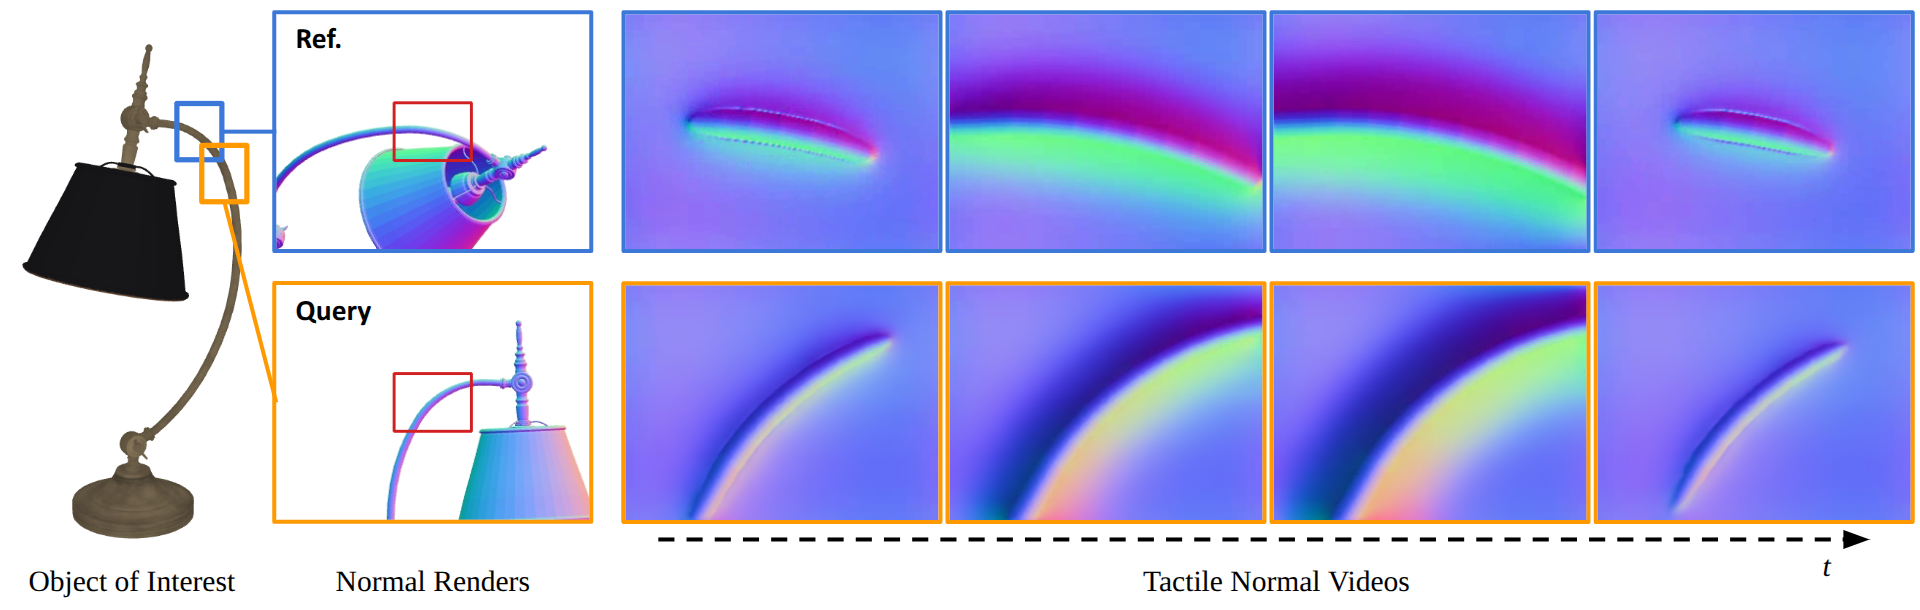
\includegraphics[width=\linewidth]{figures/teaser.pdf}
  \rule{\linewidth}{4.2cm}% PLACEHOLDER -- remove when the real figure is dropped in
  \caption{\textbf{Tactile analogies.} Given a reference touch recorded on an object (top right)
    together with the surface geometry at the location it was taken from (top left), we predict
    the tactile signal that the sensor would measure at a new, previously untouched location
    (bottom right) given only the geometry there (bottom left). We represent a touch as a
    \emph{tactile normal video}, which records how the sensor's deformable gel bends over the
    course of a press, so the prediction is a short video rather than a single frame. The
    relationship between the two columns is the analogy our method must transfer: as the reference
    geometry is to the reference touch, so the query geometry is to the touch we synthesise.}
  \label{fig:teaser}
\end{figure}
